% !TEX encoding = UTF-8
% !TEX TS-program = pdflatex
% !TEX root = ../tesi.tex

%**************************************************************
\chapter{Introduzione}
\label{cap:introduzione}
%**************************************************************
In questo capitolo viene presentata, brevemente, l'azienda e la sua metodologia di lavoro che utilizza per lo sviluppo dei suoi progetti.\\
Verrà successivamente illustrato, in modo dettagliato, il progetto affrontato durante il periodo di stage partendo da una visione generale del problema ed arrivando alle possibili soluzioni studiate.

%**************************************************************
\section{L'azienda}
\subsection{Profilo aziendale}
Athesys nasce nel 2010 con sede a Padova dall’unione di professionisti IT che vantano una lunga esperienza in diversi ambiti tecnologici con l’obiettivo di mettere a fattor comune la loro competenza e tradurla nella capacità di erogare consulenza ad elevato contenuto tecnologico e progettuale a supporto delle complesse scelte strategiche che le aziende sono chiamate a prendere con sempre maggiore rapidità\cite{athesys}.\\
I settori in cui l'azienda si muove sono diversi:
\begin{itemize}
	\item \textit{Identity and Access Management} - propone, alle aziende clienti, soluzioni per effettuare il controllo degli accessi alle applicazioni aziendali e di gestire il ciclo di vita degli account applicativi;
	\item \textit{Database Management} - aiuta le aziende a progettare i database più adatti alle loro esigenze focalizzandosi sull'alta affidabilità e scalabilità;
	\item \textit{Business Intelligence} - propone alle aziende di raccogliere, da più sorgenti, le informazioni complesse e renderle fruibili attraverso report personalizzabili e dashboard intuitive. La Business Intelligence può migliorare le prestazioni delle imprese grazie a:
	\begin{itemize}
		\item generazione di report che migliorano l'efficenza operativa e la visibilità del business aziendale;
		\item ottimizzazione del ritorno d'investimento in ambito IT grazie a sistemi di \emph{\gls{DataManagement}}\glsfirstoccur, \emph{\gls{DataMining}}\glsfirstoccur, e pianificazione delle risorse;
		\item miglioramento delle performance delle procedure per la decisione delle strategie aziendali.
	\end{itemize} 
\end{itemize}
Athesys S.r.l. lavora presso importanti realtà aziendali, operanti nel settore bancario, pubblico ed automotive.\\
La sua missione è quella di garantire al proprio cliente un lavoro ad alto valore professionale con un costante e affidabile supporto; ed è per questo che l'azienda ha rinnovato il proprio certificato ISO9001 dimostrando un controllo maggiore sui propri processi interni.\\

\begin{figure}[!h]
	\centering
	
\includegraphics{immagini/logo_athesys}
	\caption{Logo Athesys S.r.l}
\end{figure}

\subsection{Metodologia di lavoro}

\begin{figure}[!h]
	\centering
	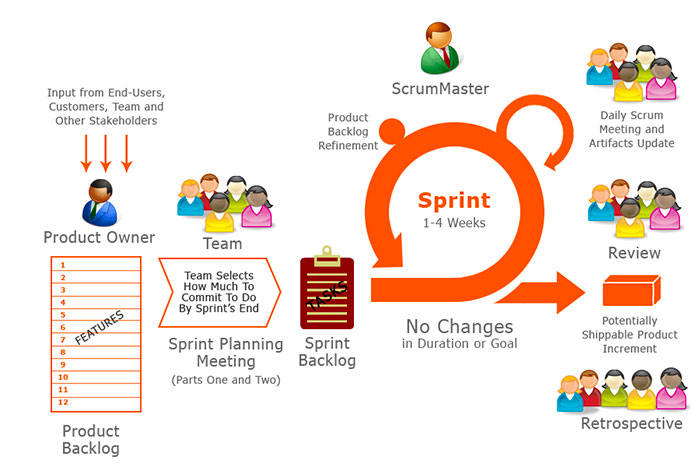
\includegraphics[scale=0.35]{immagini/scrum}
	\caption{Schema Scrum}
\end{figure}

Il team aziendale viene gestito secondo la metodologia \emph{\gls{Scrum}}\glsfirstoccur, framework \emph{\gls{agile}}\glsfirstoccur di sviluppo del sofware, introdotto nel 1995 da Ken Schwaber e Jeff Sutherland. Tale modello si basa sulla teoria del controllo empirico del processo la quale afferma che la conoscenza deriva da decisioni di esperienza e che la preparazione si basa su ciò che è già noto. \textit{Scrum}, dunque, prevede un approccio iterativo e incrementale per cercare di ottimizzare la prevedibilità e il controllo dei rischi. Sono tre i principi che sostengono la teoria del controllo empirico del processo:
\begin{enumerate}
	\item \textbf{Trasparenza} - i responsabili devono avere una visione degli aspetti più significativi del processo per poter monitorare il risultato del lavoro che sia conforme alle attese;
	\item \textbf{Ispezione} - il lavoro di uno \textit{sprint} deve poter essere ispezionato per rilevare variazioni indesiderate rispetto all'obiettivo;
	\item \textbf{Adattamento} - se durante un'ispezione viene riscontrato uno o più aspetti che si discostano dai limiti accettabili e il prodotto risulta inacettabile, il processo in esecuzione deve essere adattato e questo deve avvenire nel minor tempo possibile al fine di evitare ulteriori deviazioni.
\end{enumerate}
Il punto centrale dello \textit{Scrum} è dato dallo \textit{sprint}, esso può essere considerato come un progetto con la durata massima di 4 settimane nelle quali deve essere portato a termine e che, alla sua conclusione, porterà ad un incremento del prodotto. Durante uno \textit{sprint} non vengono apportate modifiche che potrebbero minarne l'esistenza del prodotto, inoltre gli obiettivi di qualità non devono diminuire mentre, l'ambito di applicazione del progetto, può essere chiarito e rinegoziato tra team di sviluppo e \textit{stakeholders}. Nel modello \textit{Scrum} i requisiti, le funzionalità, i miglioramenti e le correzioni sono ordinati all'interno del \emph{\gls{ProductBacklog}}\glsfirstoccur; esso non è mai completo, è dinamico ed evolve con il prodotto.\\
Lo \emph{\gls{SprintBacklog}}\glsfirstoccur, invece, è una previsione redatta in sede di riunione dal team di sviluppo con gli obiettivi che deve raggiungere lo \textit{sprint} e il lavoro che ne deriva anche in termini di tempo.\\
Lo \gls{SprintBacklog} aiuta, quindi, a rendere trasparente il lavoro necessario per raggiungere gli obiettivi dello \textit{sprint}.
Athesys adotta \textit{sprint} di durata quindicinale, preceduti da riunioni per defnire gli obiettivi e i tempi dello \textit{sprint} tra i membri del team di sviluppo. Ad ogni \textit{sprint} ne segue la sua ispezione e in caso l'adattamento con miglioramenti e correzioni.





%**************************************************************
\section{L'idea}

Introduzione all'idea dello stage.

%**************************************************************
